%
% elliptic.tex -- Boundary conditions for elliptic PDE
%
% (c) 2019 Prof Dr Andreas Müller, Hochschule Rapperswil
%
\documentclass[tikz,12pt]{standalone}
\usepackage{amsmath}
\usepackage{times}
\usepackage{txfonts}
\usepackage{pgfplots}
\usepackage{csvsimple}
\usetikzlibrary{arrows,intersections,math}
\begin{document}
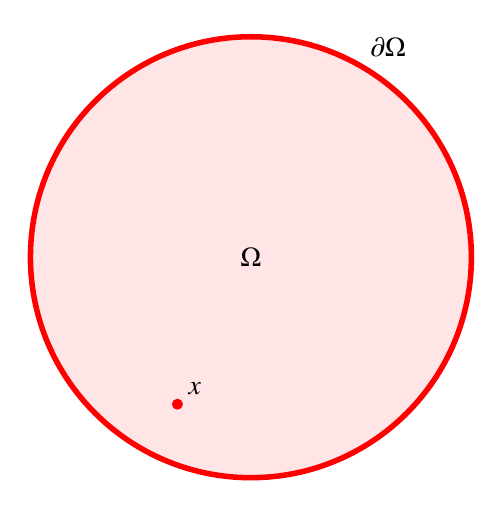
\begin{tikzpicture}[>=latex]

\def\radius{2.8}

\fill[color=red!10] (0,0) circle[radius={\radius}];
\draw[color=red,line width=2.0pt] (0,0) circle[radius={\radius}];

\node at (0,0) {$\Omega$};

\coordinate (A) at ({(\radius/3)*(-1)},{(\radius/3)*(-2)});

\fill[color=red] (A) circle[radius=2.0pt];
\node at (A) [above right] {$x$};
\def\a{60}
\node at ({\radius*cos(\a)},{\radius*sin(\a)}) [above right] {$\partial\Omega$};

\end{tikzpicture}
\end{document}

